\documentclass[]{article}

\usepackage[]{graphicx}

\newcommand{\code}[1]{\texttt{#1}}

\title{The Yi Text Editor}

\author{Don Stewart}

\begin{document}

\maketitle

\section{Writing a custom keymap}

Writing your own keymap is fairly easy. Here's how to use the example
Nano.hs keymap:
\begin{verbatim}
    $ cp examples/Config.hs ~/.yi/
    $ cp Yi/Keymap/Nano.hs ~/.yi

    Now edit ~/.yi/Config.hs to use ~/.yi/Nano.hs
    you need to replace:
                "import qualified Keymap"
           with "import qualified Nano"

           and  "keymap = Keymap.keymap"
           with "keymap = Nano.keymap"
\end{verbatim}

and you're done. \texttt{:reload} will then dynamically load the new
keymap. Keymaps are written as \code{[Char] -> [Action]} lexers, and
complicated lexers are best constructed using the \code{Yi/Lexers}
library, which uses the Ctk lazy lexer combinators to specify
dynamically-modifiable lexer tables.

\section{Runtime}

\subsection{Configuration}

Preferences are stored in \code{\$HOME/.yi/Config.hs}, and written in
Haskell. Look in examples/ for example Config.hs. If the
\code{\$HOME/.yi} directory doesn't exist, yi uses \code{Yi/Yi.hs} for
the defaults, this is also what is used in yi-static.

To get at yi internals from your config script, either import Yi.Yi,
which brings most of the commonly used modules into scope, or explicitly
import something from \code{Yi/*}. You can read the haddock-generated
docs for some API details. Generate them with \code{make html}.

\subsection{Plugin architecture}

All configuration takes place via dynamically loaded Haskell modules.
Additionally, the editor itself is a dynamically loaded library,
allowing us to implement \code{:reboot}, such that you can edit the
editor itself, and reload it, without having to quit the editor.

The boot process is as follows:

\begin{verbatim}
           Boot.hs + Config.hs
                   |
                 Yi.o
                   |
                HSyi.o (-package yi)
\end{verbatim}

The boot loader module dynamically loads any config files, and their
dependencies, and passes the config value to the top level module of the
editor package (Yi.o). It also passes the reload and reboot functions,
so that the editor is able to jump back to the boot loader and unload
itself. Boot.main jumps to Yi.dynamic\_main. It is Yi.o that then
performs argument checks, and initialises the editor, before jumping to
the editor main loop. When Yi is built the \code{static} way, we skip
the boot loader, and instead start at \code{Main.main}. The structure of
yi can be seen in Figure \ref{overview}.

% flow-diagram of how from source to Haskell value
\begin{figure}
  \begin{center}
    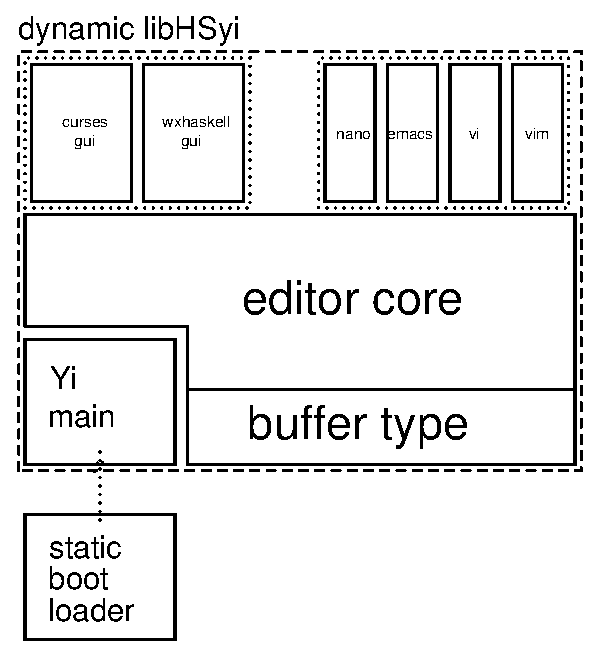
\includegraphics[scale=0.7]{yi_overview.eps}
    \caption{Structure of yi}
    \label{overview}
  \end{center}
\end{figure}
%

\section{Components}

The undo library is based on the restricted, linear undo described in
~\cite{berlage94selective}.

\section{Build system}

Extra arguments can be passed at runtime as: make HC\_OPTS=-ddump-minimal-imports

\subsection{Profiling}

You can build yi-static for profiling. Just set:
\begin{verbatim}
    make way=p
\end{verbatim}
and then invoke
\begin{verbatim}
    ./yi-static +RTS -p
\end{verbatim}
and once you quit you'll get a \code{yi-static.prof} file with profiling
statistics.

\section{Development}

\subsection{Style guide}

Please make sure you code compiles with -Wall -Werror -fno-glasgow-exts
(we're trying to support nhc98). Use Haddock markup to document any
functions that are exported -- user's may want to use this code at some
point. We use CPP to pass platform specific options into files. Please
provide explicit import lists where reasonable, and keep imports in some
sorted order. Please don't introduce POSIX dependencies.

\subsection{GHCi}

You can actually run this stuff in GHCi! To just run yi-core (the GUI
etc, without worrying about booting the thing):

{\small
\begin{verbatim}
        ghci -package-conf yi.conf -package yi
        manzano$ ghci -package-conf yi.conf -package yi
           ___         ___ _
          / _ \ /\  /\/ __(_)
         / /_\// /_/ / /  | |      GHC Interactive, version 6.3, for Haskell 98.
        / /_\\/ __  / /___| |      http://www.haskell.org/ghc/
        \____/\/ /_/\____/|_|      Type :? for help.

        Loading package base ... linking ... done.
        Loading package haskell98 ... linking ... done.
        Loading package mtl ... linking ... done.
        Loading package lang ... linking ... done.
        Loading package unix ... linking ... done.
        Loading package posix ... linking ... done.
        Loading package yi ... linking ... done.
        Prelude> :l Main
        Prelude Main> main
\end{verbatim}
}

To run the whole thing is a bit harder, and requires faking the package
lib flags in yi.conf (leave off the last 2 arguments if you're on Linux). And
if we haven't installed it yet (you want to run in-tree), then you have
to set the command line arguments. Also, to do this trick you need ghc-6.2.2
or greater, which contain appropriate RTS patches for running dynamic
loaders dynamically.

{\small
\begin{verbatim}
        manzano$ ghci -package plugins -liconv -L/usr/local/lib
           ___         ___ _
          / _ \ /\  /\/ __(_)
         / /_\// /_/ / /  | |      GHC Interactive, version 6.3, for Haskell 98.
        / /_\\/ __  / /___| |      http://www.haskell.org/ghc/
        \____/\/ /_/\____/|_|      Type :? for help.

        Loading package base ... linking ... done.
        Loading package altdata ... linking ... done.
        Loading package haskell98 ... linking ... done.
        Loading package hi ... linking ... done.
        Loading package unix ... linking ... done.
        Loading package haskell-src ... linking ... done.
        Loading package mtl ... linking ... done.
        Loading package lang ... linking ... done.
        Loading package posix ... linking ... done.
        Loading package plugins ... linking ... done.
        Loading object (dynamic) iconv ... done
        final link ... done
    Prelude> :set -DLIBDIR="/usr/local/lib/yi"
    Prelude> :set args -B/home/dons/src/projects/yi
    Prelude> :l Boot.hs
    *Boot>
        Prelude Boot> main
        Starting up dynamic Haskell ... jumping over the edge ... done.
\end{verbatim}
}

For example, to modify \code{\$(TOP)/Yi.hs} in GHCi, you would:

{\small
\begin{verbatim}
        manzano$ ghci -package-conf yi.conf -package yi
        Prelude> :l Yi.hs
        *Yi> :t dynamic_main
        dynamic_main :: Maybe ConfigData -> IO ()
        *Yi> :reload
        Compiling Yi           ( Yi.hs, interpreted )
\end{verbatim}
}

\section{Porting to other compilers}

To use nhc98 (some more porting required). The best we can do is
yi-static:
\begin{verbatim}
    ./configure --with-hc=nhc98
    gmake
\end{verbatim}

We have 3 problems:
\begin{itemize}
    \item We rely on some non-nhc98 libraries: MVar, threads, Unique..
    \item We use hsc2hs for FFI files
    \item There's still files which use GHC extensions
\end{itemize}

The big problem is the extra libraries.

\bibliographystyle{abbrv}
\bibliography{yi}

\end{document}

